\begin{figure}[!ht]
    \centering
    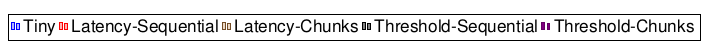
\includegraphics[scale=0.3]{images/legend}
    
    \subfloat[Tempo de execução]{
        \label{Kmeans}
        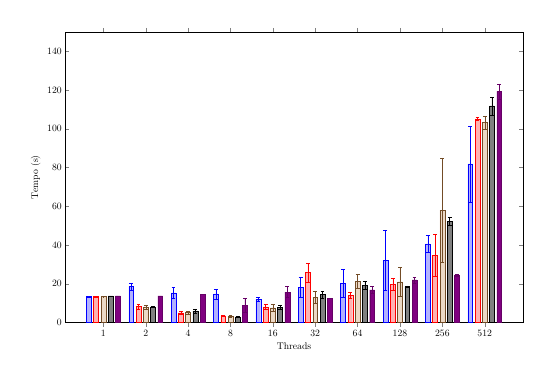
\begin{tikzpicture}[scale=0.35, baseline]
        \begin{axis}[
            width=1.5 \linewidth,
            height=1 \linewidth,
            %media de tempo intruder
            ybar=2.5pt,
            %enlargelimits=0.10,
            % legend style={at={(0.5,-0.15)}, anchor=north, legend columns=-1},
            ylabel=Tempo (s),
            xlabel=Threads,
            symbolic x coords={1, 2, 4, 8, 16, 32, 64, 128, 256, 512},
            xtick=data,
            ymin=0,
            ymax=150,
            bar width=5pt,
            % nodes near coords,
            nodes near coords align={vertical},
        ]
        \addplot+[error bars,y dir=both, y explicit] coordinates {
            (1,13.32)+-(1,0.05) (2,18.64)+-(2,1.86) (4,15.33)+-(4,2.68) (8,14.72)+-(8,2.44) (16,12.06)+-(16,0.95) (32,18.24)+-(32,5.19) (64,20.20)+-(64,7.21) (128,32.16)+-(128,15.30) (256,40.54)+-(256,4.28) (512,81.86)+-(512,19.67) 
        };
        \addplot+[error bars,y dir=both, y explicit] coordinates {
            (1,13.36)+-(1,0.05) (2,8.25)+-(2,1.41) (4,5.05)+-(4,0.53) (8,3.49)+-(8,0.45) (16,8.10)+-(16,1.15) (32,25.81)+-(32,4.77) (64,14.01)+-(64,1.61) (128,19.77)+-(128,3.11) (256,34.76)+-(256,10.90) (512,105.07)+-(512,0.66)
        };
        \addplot+[error bars,y dir=both, y explicit] coordinates {
            (1,13.39)+-(1,0.03) (2,8.05)+-(2,1.09) (4,5.13)+-(4,0.64) (8,3.37)+-(8,0.57) (16,7.62)+-(16,1.79) (32,13.01)+-(32,3.05) (64,21.35)+-(64,3.62) (128,21.05)+-(128,7.45) (256,57.98)+-(256,27.06) (512,103.22)+-(512,3.24)
        };
        \addplot+[error bars,y dir=both, y explicit] coordinates {
            (1,13.70)+-(1,0.00) (2,8.08)+-(2,0.39) (4,6.03)+-(4,1.01) (8,2.85)+-(8,0.20) (16,7.92)+-(16,1.01) (32,14.57)+-(32,1.81) (64,19.24)+-(64,2.21) (128,18.49)+-(128,0.48) (256,52.31)+-(256,2.27) (512,111.88)+-(512,4.66) 
        };
        \addplot+[error bars,y dir=both, y explicit] coordinates {
            (1,13.73)+-(1,0.00) (2,13.72)+-(2,0.00) (4,14.49)+-(4,0.02) (8,8.98)+-(8,3.78) (16,15.66)+-(16,2.82) (32,12.59)+-(32,0.01) (64,16.86)+-(64,1.83) (128,21.99)+-(128,1.45) (256,24.41)+-(256,0.44) (512,119.27)+-(512,3.89)
        };
        % \legend {Tiny, Latency-Sequential, Latency-Chunks, Threshold-Sequential, Threshold-Chunks}
        \end{axis}
        \end{tikzpicture}
    }
    \subfloat[Aborts]{
        \label{abortKmeans}
        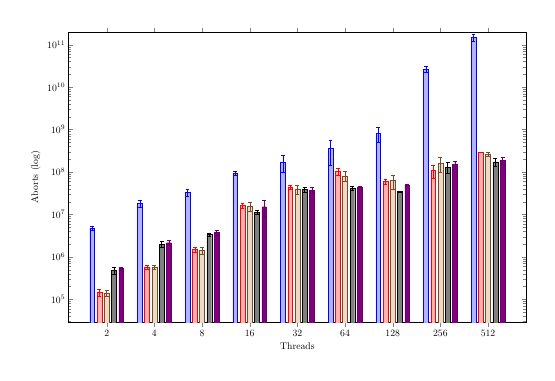
\begin{tikzpicture}[scale=0.35, baseline]
        \begin{axis}[
            ymode=log,
            width=1.5 \linewidth,
            height=1 \linewidth,
            %media de tempo intruder
            ybar=2.5pt,
            %enlargelimits=0.10,            
            % legend style={at={(0.45,1.1)}, anchor=south, legend columns=-1},
            ylabel=Aborts (log),
            xlabel=Threads,
            symbolic x coords={1, 2, 4, 8, 16, 32, 64, 128, 256, 512},
            xtick=data,
            ymin=0,
            ymax=200000000000,
            bar width=5pt,
            % nodes near coords,
            nodes near coords align={vertical},
        ]
        \addplot+[error bars,y dir=both, y explicit] coordinates {
            (1,0.0)+-(1,0.0) (2,4797421.2)+-(2,479774.7418784778) (4,18101846.8)+-(4,3591708.3539415835) (8,33182746.2)+-(8,6732288.556793311) (16,93057923.8)+-(16,9863144.322012922) (32,171442797.6)+-(32,74829388.10384364) (64,359745893.2)+-(64,213043475.04545623) (128,807753260.2)+-(128,310719932.9857997) (256,26569175006.4)+-(256,4470117158.120106) (512,146296330743.6)+-(512,26886172215.929005) 
        };
        \addplot+[error bars,y dir=both, y explicit] coordinates {
            (1,0.0)+-(1,0.0) (2,144295.6)+-(2,24864.282793597726) (4,579330.6)+-(4,68221.2484981036) (8,1486520.2)+-(8,200173.524986098) (16,16580311.4)+-(16,2227873.6890443857) (32,45063610.6)+-(32,5053643.0020858655) (64,103498202.6)+-(64,18052939.09375) (128,59441333.6)+-(128,8917614.717479235) (256,109146323.8)+-(256,36880499.382352196) (512,294773353.4)+-(512,3281309.7536428105)
        };
        \addplot+[error bars,y dir=both, y explicit] coordinates {
             (1,0.0)+-(1,0.0) (2,141609.1)+-(2,19957.913370139675) (4,570320.1)+-(4,69142.6626511447) (8,1412101.5)+-(8,239771.55806068826) (16,15454899.8)+-(16,3814349.1856658272) (32,39591108.222222224)+-(32,9286948.71968007) (64,81659510.1)+-(64,21584431.489666473) (128,62701912.9)+-(128,22625798.149042867) (256,157892521.1)+-(256,60541141.358650364) (512,267641468.75)+-(512,32356420.707834) 
        };
        \addplot+[error bars,y dir=both, y explicit] coordinates {
            (1,0.0)+-(1,0.0) (2,489474.6)+-(2,95557.56667391652) (4,1982817.6)+-(4,324496.7328282983) (8,3338695.4)+-(8,339537.1836017964) (16,11407592.4)+-(16,1467579.9615602007) (32,38923440.666666664)+-(32,5311247.22872386) (64,42424191.0)+-(64,4907763.0) (128,34826711.0)+-(128,578473.0) (256,128783746.63)+-(256,37482783.86) (512,173847878.28)+-(512,37384778.0)
        };
        \addplot+[error bars,y dir=both, y explicit] coordinates {
            (1,0.0)+-(1,0.0) (2,528574.7)+-(2,29384.0) (4,2157923.0)+-(4,283746.0) (8,3736425.62)+-(8,429388.0) (16,15208687.0)+-(16,6397145.233711557) (32,37279545.0)+-(32,6425946.0) (64,43456253.0)+-(64,3849829.0) (128,49875516.0)+-(128,675193.0) (256,148983127.32)+-(256,31827833.0) (512,187678278.0)+-(512,32738943.73)
        };
        % \legend {Tiny, Latency-Sequential, Latency-Chunks, Threshold-Sequential, Threshold-Chunks}
        \end{axis}
        \end{tikzpicture}
    }
\end{figure}
